\documentclass{beamer}
%\usepackage{beamerthemesplit}
\mode<presentation>
\usetheme{Montpellier}
\usepackage{graphicx,amssymb,amsmath,amsthm,bm}
\usepackage{caption}

\title{Homework 4 - Results}

\author{}
\institute[]{}

\begin{document}



\frame{
\titlepage
}

\section{Introduction}

\begin{frame}{Likelihood Function}
\begin{align}
l_i^1 = \int [\Pi_t \frac{1}{\sigma_{1t}} \phi(\frac{y_{it1} - X_{it1}\beta_1 - \theta_i}{\sigma_{1t}})]\Phi(\frac{\sum_t (X_{it1} - X_{it0})\tilde{\beta} - Z_i \delta - \theta_i \gamma}{\sigma_w}) \\
 \frac{1}{\sqrt{2 \pi} \sigma_\theta} \exp(- (\frac{\theta_i}{\sqrt{2}\sigma_\theta})^2) d\theta
\end{align}
\begin{itemize}
\item Use Gauss-Hermite to approximate integral. Change of variables necessary.
\end{itemize}
\end{frame}

\begin{frame}{Test on fake data first}
\centering
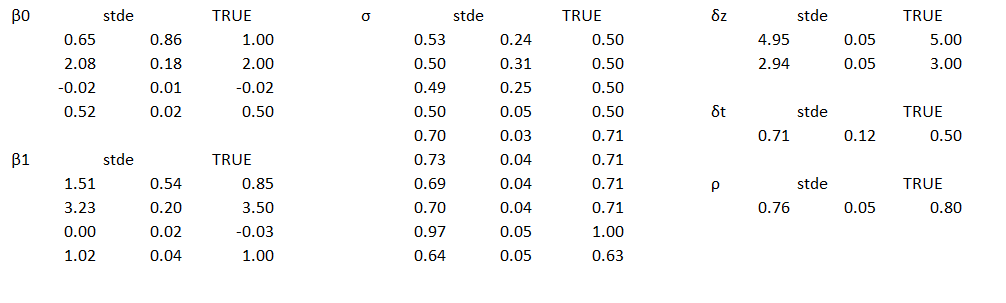
\includegraphics[scale=0.55]{fake_est.png}
\end{frame}

\begin{frame}{Test on fake data first}
\centering
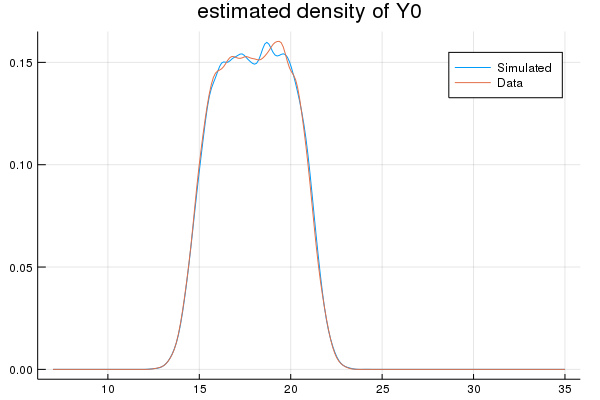
\includegraphics[scale=0.5]{y0_fake.png}
\end{frame}
\begin{frame}{Test on fake data first}
\centering
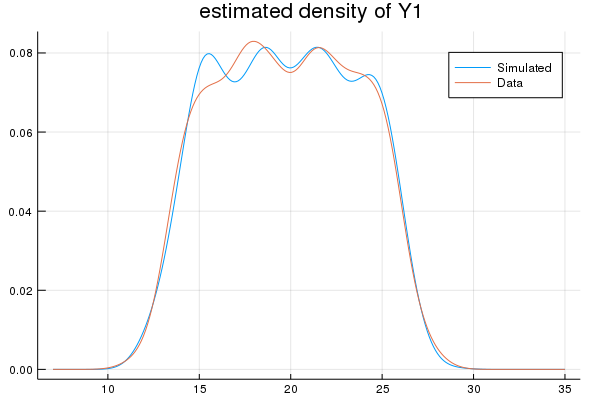
\includegraphics[scale=0.5]{y1_fake.png}
\end{frame}

\begin{frame}{Test on fake data first}
\begin{itemize}
\item Mean school choice: Data = 0.367; Simulated = 0.366
\end{itemize}
\end{frame}

\begin{frame}{Summary stats of zb}
\centering
Mean:           0.020392

Minimum:        -2.929359

1st Quartile:   -0.628405

Median:         0.002442

3rd Quartile:   0.619182

Maximum:        2.957066
\end{frame}

\begin{frame}{Test on fake data first}
\begin{itemize}
\item New Mean school choice: 0.217
\end{itemize}
\end{frame}

\begin{frame}{Estimates in log-units}
\begin{itemize}
\item ATE = 11.49
\item ATT = 8.12
\item LATE = 8.46
\end{itemize}
\end{frame}


\begin{frame}{NLSY data}
\begin{itemize}
\item X = experience, experience2 and family income
\item Z = tuition, family income, numsibs, scores, mother and father education
\end{itemize}
\end{frame}

\begin{frame}{Likelihood Function}
\begin{align}
\Phi(\frac{Xs_{1i}\tilde{\beta} + (exp_{s=1,i} - exp_{s=0,i})\tilde{\beta} + (exp^2_{s=1,i} - exp^2_{s=0,i})\tilde{\beta} + Xs^4_{i}\tilde{\beta} - Z_i \delta - \theta_i \gamma}{\sigma_w}) \\
\end{align}
\centering
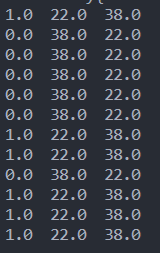
\includegraphics[scale=0.59]{xsb_example.png}
\end{frame}

\begin{frame}{NLSY data}
\begin{itemize}
\item Initial guesses:
\item OLS on each wage equation, probit on Zs, standard errors from OLS
\item probit on Xs, Zs, but experience is a perfect predictor!
\end{itemize}
\end{frame}

\begin{frame}{What I tried}
\begin{itemize}
\item X = experience, experience2 and family income
\item Z = tuition, family income, numsibs, scores, mother and father education
\item If I take the log(10000*income) and tuition, standard errors blow up to 1e10 on $\delta_Z$ and $\sigma_w$, very low variaton may be cause
\item If i just multiply family income and tuition by $10^a, a=1,2,3,4$, model doesn't converge
\item Same thing happens by removing family income from Z
\item Same thing happens by permutating with numsbis, scores, mother and father educ.
\end{itemize}
\end{frame}


\begin{frame}{NLSY Estimates}
\centering
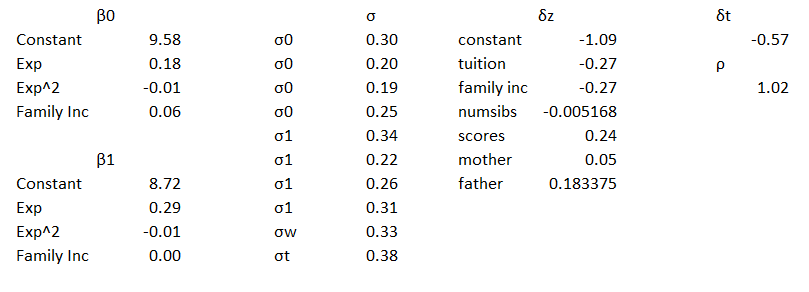
\includegraphics[scale=0.59]{nlsy_est.png}

No standard errors :(
\end{frame}

\begin{frame}{NLSY fit}
\centering
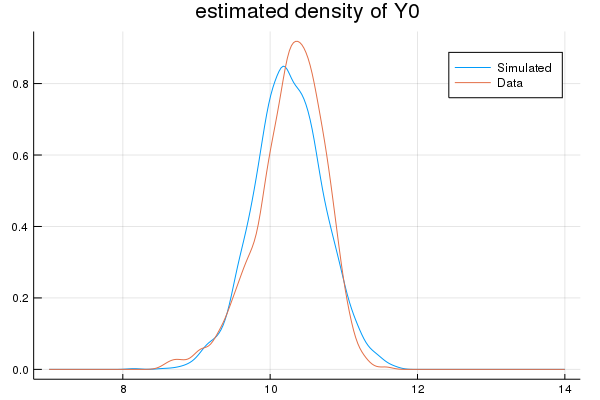
\includegraphics[scale=0.5]{y0.png}
\end{frame}
\begin{frame}{NLSY fit}
\centering
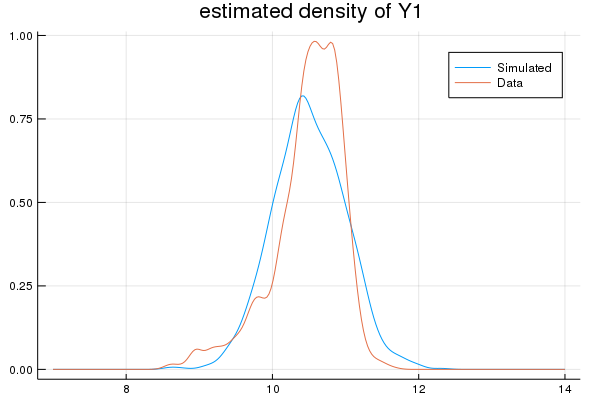
\includegraphics[scale=0.5]{y1.png}
\end{frame}

\begin{frame}{NLSY fit}
\begin{itemize}
\item Mean school choice: Data = 0.372; Simulated = 0.372!
\end{itemize}
\end{frame}






\begin{frame}{Summary stats of tuition}
\centering
Mean:           0.214001

Minimum:        0.000000

1st Quartile:   0.159418

Median:         0.207967

3rd Quartile:   0.257659

Maximum:        0.522191
\end{frame}


\begin{frame}{Estimates}
\begin{itemize}
\item So, I will zero tuition for those below the mean
\item New mean school choice: 0.372!
\end{itemize}
\end{frame}

\begin{frame}{Summary stats sim y0}
\centering
Mean:           31,645.128

Minimum:        4,904.970

1st Quartile:   20,792.095

Median:         28,934.711

3rd Quartile:   39,456.350

Maximum:        155,488.773
\end{frame}

\begin{frame}{Summary stats sim y1}
\centering
Mean:           29,664.918

Minimum:        3,547.429

1st Quartile:   17,553.850

Median:         25,781.921

3rd Quartile:   37,211.698

Maximum:        152,681.450
\end{frame}

\begin{frame}{Estimates}
\begin{itemize}
\item ATE = -1,980.21
\item ATT = 8,623.56
\item LATE = ?
\end{itemize}
\end{frame}


\end{document}